\documentclass[conference]{IEEEtran}
\IEEEoverridecommandlockouts
% The preceding line is only needed to identify funding in the first footnote. If that is unneeded, please comment it out.
%Template version as of 6/27/2024

\usepackage{cite}
\usepackage{amsmath,amssymb,amsfonts}
\usepackage{algorithmic}
\usepackage{graphicx}
\usepackage{subcaption}
\usepackage{textcomp}
\usepackage{xcolor}
\usepackage[automake=immediate,abbreviations,symbols]{glossaries-extra}
\setabbreviationstyle{long-short}
\loadglsentries{acronyms.tex}
\makeglossaries
\def\BibTeX{{\rm B\kern-.05em{\sc i\kern-.025em b}\kern-.08em
    T\kern-.1667em\lower.7ex\hbox{E}\kern-.125emX}}
\begin{document}

\title{Guided Genetic Algorithm for Optimising Camera Placement in a Motion Capture System\\
\thanks{Identify applicable funding agency here. If none, delete this.}
}

\author{\IEEEauthorblockN{1\textsuperscript{st} Shannon Pitman}
\IEEEauthorblockA{\textit{University of Cape Town Mechanical Engineering Department} \\
\textit{Mechatronic.SystemsGroup}\\
Cape Town, South Africa \\
ptmsha001@uct.ac.za}
\and
\IEEEauthorblockN{2\textsuperscript{nd} Arnold Pretorius}
\IEEEauthorblockA{\textit{University of Cape Town Mechanical Engineering Department} \\
\textit{Mechatronic.SystemsGroup}\\
Cape Town, South Africa\\
arnold.pretorius@uct.ac.za}
}

\maketitle

\begin{abstract}
This document is a model and instructions for \LaTeX.
This and the IEEEtran.cls file define the components of your paper [title, text, heads, etc.]. *CRITICAL: Do Not Use Symbols, Special Characters, Footnotes,
or Math in Paper Title or Abstract.
\end{abstract}

\begin{IEEEkeywords}
Genetic Algorithm, Optimisation, Motion Capture, Resolution Uncertainty, Probabalistic Dynamic Occlusion
\end{IEEEkeywords}

\section{Introduction}
\label{sec: Introduction}
The quality of a multi-camera tracking system is determined as much by the geometric arrangement of its sensors as by the hardware itself.
Sensor noise, calibration accuracy, and algorithmic sophistication all matter; yet even a perfectly calibrated, high-quality system running a sophisticated estimator can fail to localise a target if its cameras are arranged poorly. Solving the optimal camera placement (OCP) problem requires both a model of how that error arises and an optimiser able to navigate a large search space in reasonable time.

Without a formal optimiser, camera networks are typically set-up through ad-hoc designer intuition or rule-of-thumb  guidelines, such as distributing the cameras evenly around the perimeter. While this may appear as a streamlined approach, the designer has no means of assessing whether a different arrangement would reduce localisation error or be more robust in tracking erratic trajectories that may mask the marker from line-of-sight. Therefore, the chosen configuration is neither verifiably optimal nor is the theoretical performance quantified. This is particularly pertinent when the number of cameras is constrained by budget, inherting inferiror hardware and as such each camera should be placed to contribute advantageously to the overall network.

The present work is the placement prerequisite for a wider project: a low-cost, marker-based motion-capture system that uses inexpensive
cameras to provide real-time tracking and localisation feedback to small robotic platforms, including \glspl{UAV}. A well-chosen camera arrangement absorbs a substantial part of the consequences of cheaper, and thus inferior hardware before it reaches the estimator. Two consequences follow. First, the coarser sensor makes resolution uncertainty a dominant error source, so the optimiser must explicitly minimise the geometric component of triangulation error rather than only maximising visibility of the entire capture volume. Second, because \gls{UAV} in particular execute unanticipated, agile manoeuvres in which the frame itself can occlude markers from one or more cameras simultaneously, the optimiser must be robust to dynamic occlusion over an agnostic platform and trajectory. Together these requirements motivate a composite cost function that penalises both error sources.

The geometric mechanism behind resolution uncertainty is straightforward. Each camera discretises its viewport into pixels; the target's true position lies somewhere inside the pixel onto which it projects. Back-projected, that pixel becomes a four-sided pyramid in three dimensions, and the intersection of the pyramids from all observing cameras bounds the recoverable position \cite{sharma_analysis_1998}. The shape of that intersection depends entirely on where the cameras sit: near-parallel viewing angles produce a long error region along the depth axis, while well-separated angles produce a compact error region with ultimately less uncertainty. The second main source of failure in optical measurements is dynamic occlusion: when fewer than two cameras retain line of sight to a marker, triangulation fails and the trajectory estimator can only rely on predictions. Rahimian and Kearney illustratd the effectiveness of compensating for this when optimising their network of OptiTrack cameras: on a fixed $37$-marker capture, re-optimising the position of the same cameras
raised full-marker reconstruction from $30\,\%$ of frames to $86\,\%$ \cite{rahimian_optimal_2017}. The cameras, the calibration,
and the subject were unchanged; only the arrangement was different.

The cost function we construct from these two mechanisms is non-differentiable (a visibility step exists at every field-of-view
boundary), non-convex (small camera displacements switch which cameras contribute to a marker's uncertainty region), and multimodal (different arrangements achieve comparable quality through qualitatively different geometries). Gradient-based interior-point solvers can be made to work by smoothing the visibility test, but then descend the surrogate rather than the true physical objective. Binary-integer formulations linearise at the cost of discretising the placement space and bounding the modelling fidelity. A population-based, derivative-free optimiser avoids both constraints. Section \ref{sec:ga} formalises this choice and introduces the operators that adapt a real-coded GA to the geometry of camera placement.

This paper contributes the following.
\begin{enumerate}
\item A guided perimeter initialisation that locates every camera on a mountable wall face of the workspace and orients it toward a balanced grid of section centres based on the amount of available cameras, so that no chromosome in the initial population contains a geometrically invalid camera positions and their predisposed orentations are balanced to view the majority of the capture volume.
\item A camera-block-aware double-point crossover that exchanges complete six-gene camera blocks between parents. Standard gene-wise blend crossover, in our experiments, consistently produced interior-mounted cameras with arbitrary orientations and degraded convergence; the block-aware variant preserves the position and orientation coupling that makes a camera useful and swaps cameras between candidates.
\item A Lamarckian camera-repair operator, applied deterministically every tenth generation and probabilistically in the intervening ones, that re-aims any camera contributing below a coverage threshold. The operator extends \textcite{aissaoui_designing_2018} initialisation-only guidance into a continuous corrective approach.
\item A dual-modality discretisation: a single algorithm produces a UAV-tuned (full-volume) and a UGV-tuned (ground-slab) configuration by altering only the target-point grid.
\end{enumerate}

We do not, in this paper, report physical deployment of the resulting configurations. The simulation results we present are sufficient to demonstrate that the optimiser is well-behaved and that the headline improvement is large; the hardware comparison is the subject of future work. Section \ref{sec:related} positions the method against the foundations it draws on; Section \ref{sec:formulation} defines the cost function; Section \ref{sec:ga} the optimisation algorithm; Section \ref{sec:setup} the experimental setup; Section \ref{sec:results} the results; and Section \ref{sec:conclusion} concludes and elucidates next steps.

\section{Related Work}
\label{sec:related}
The optimal sensor placement literature is substantial; not all of it informs the design presented here. This section identifies the works that directly shape our cost function and algorithm, and reports any inheritance as as the limitations.

\subsection{Cost-function Foundations}

The pyramid-intersection uncertainty model originates with Wu, Sharma, and Huang \cite{sharma_analysis_1998}, who treated the half-pixel quantisation interval as a square (pixel-length) error region in image space, back-projected its four corners into a four-sided world-space pyramid, and bounded the recoverable target position by the intersection of these pyramids across observing cameras. Their final scalar uncertainty measure was the volume of an ellipsoid fitted to the intersection vertices via an iterative downhill simplex search. The geometric content of that derivation is the only clear description of degredation loss due to resolution in the literature and we adopt it in full; the iterative fit is not, and Section \ref{sec:formulation} replaces it with a closed-form eigenvalue summation that yields a comparable quantity from a single $3\!\times\!3$ decomposition.

The probabilistic dynamic-occlusion model is built from Chen and Davis' foundation \cite{chen_camera_2000}, refined with extensive empirical validation by the same authors in 2008 \cite{chen_occlusion_2008}. Their key argument is one we adopt verbatim: when the geometry and movement of dynamic occluders is unknown at design time, the worst-case occluder must be modelled as an infinite vertical plane adjacent to the marker, with uniformly distributed orientation. This is the worst-case scenario. Their original metric estimated, by Monte Carlo sampling of occluder angles, the probability that at least two cameras retain line of sight. Significantly, their metric counts cameras; it does not interrogate their triangulability.

Rahimian and Kearney \cite{rahimian_optimal_2017} addressed that shortfall. They retained Chen and Davis's adjacent-plane occluder but imposed two constraints absent from the original: a convergence-angle bound of $[40^\circ, 140^\circ]$ on every triangulable pair (justified by the error analysis of Olague and Mohr \cite{olague_optimal_2002}), and a binary cut-off on each camera's effective marker detection range. They further observed that the projected horizontal view-vectors of $n$ cameras partition the occluder-orientation space into exactly $2n$ sectors of constant visibility, allowing the expensive Monte Carlo step to be replaced by an exact summation over sectors. We adopt the angular-sectoring formulation in full. Where we differ is in the surrounding optimiser: Rahimian and Kearney drove their cost function with simulated annealing, which they justified on the grounds that SA's probabilistic acceptance escapes the local minima endemic to non-convex visibility landscapes. The justification is sound, but it generalises: a population-based GA escapes the same minima while exposing the cost function to more diverse candidate arrangements, not just neighbouring solutions in parallel.

\subsection{Algorithmic Foundations}

Two real-coded GA precedents inform the operators in Section \ref{sec:ga}. Olague and Mohr \cite{olague_optimal_2002} encoded each camera as a continuous parameter vector and minimised the covariance of the reconstructed 3D point under stereo geometry. Their formulation is the earliest demonstration that gene-wise floating-point chromosomes are workable for OCP, and it imparts the $[40^\circ,140^\circ]$ angle bound to subsequent work via its error propagation analysis.

Aissaoui et al.\cite{aissaoui_designing_2018} reported that an unguided GA converged poorly on multi-camera MoCap problems and introduced a \emph{guided} initialisation in which the initial population of cameras was oriented towards physically plausible capture zones, estimated from expected-trajectory point clouds of a humanoid subject. The improvement was substantial in their simulation experiments both in cost and computational efficiency. Two limits in their work, by their own description, are worth naming. The first is that the guidance is applied only at initialisation; selection pressure and mutation then drive cameras anywhere the chromosome allows, including back into the geometrically invalid interior of the workspace. The second is that the validation is reported only in simulation \cite{aissaoui_designing_2018}. Our Lamarckian repair operator addresses the first limit directly; the second informs our framing of the present paper as a simulation study in its own right and places hardware deployment as future work which will be explored.

\subsection{Validation in the broader literature}
Several studies bear mention because they report real hardware trials and results. Rahimian and Kearney's experimental section, measures full-marker reconstruction averaged over captured frames across moving subjects. Chen and Davis \cite{chen_occlusion_2008} validated their occlusion metric against $256$ distinct camera configurations on a real MoCap session and reported a Pearson correlation of $0.97$ between predicted and measured occlusion against an inter-session repeatability ceiling of $0.98$. Zhao et al. \cite{zhao_approximate_2013} deployed a seven-camera surveillance network over a $7.6\!\times\!3.7\,\text{m}$ floor area to compare BIP, LP-relaxation, and greedy solvers. Ziegler et al. \cite{ziegler_optimal_2023} are an exception as they present an explicit methodology for translating optimised camera poses to physical mounting alongside their smoothed-NLP optimiser. This methodology description and the conversion step comparably to other works which leave this information and per-camera intrinsic parameters often unspecified or implicit. We will follow that protocol in the physical-validation phase in future work, as we discuss in Section~\ref{sec:conclusion}.

The remainder of the literature is dominated by simulation studies in which an optimised configuration is compared against the ad-hoc uniform baseline setup by OptiTrack in our laboratory through the cost function itself.

\section{Problem Formulation}
\label{sec:formulation}
The cost function evaluates a candidate camera configuration over a discrete target-point grid $\mathcal{T} = \{\mathbf{p}_1, \ldots, \mathbf{p}_N\}$ sampling the tracked volume. The cost has two components: resolution uncertainty arising from pixel quantisation, and dynamic occlusion arising from self-occlusion of the target. By definition the optimal design corresponds to the minimisation of this objective function.


\subsection{Resolution Uncertainty} \label{RU}
For a pinhole camera $i$ with intrinsic matrix $\mathbf{K}_i$, rotation $\mathbf{R}_i$, and centre $\mathbf{t}_i$, the four corners of the half-pixel quantisation region surrounding the projected target back-project to
\begin{equation}
\label{eq:backproject}
\mathbf{w}_{i,c} = \mathbf{R}_i\!\left(\mathbf{K}_i^{-1}\!\begin{bmatrix} u_i \pm \tfrac{1}{2} \\ v_i \pm \tfrac{1}{2} \\ 1 \end{bmatrix}\right) + \mathbf{t}_i,
\end{equation}
defining a four-sided pyramid in the world frame \cite{sharma_analysis_1998}. With $n_v \geq 2$ cameras observing $\mathbf{p}$, the intersection of their pyramids is a convex polyhedron bounding the recoverable target position.

Sharma's iterative ellipsoid fit returns a scalar uncertainty by solving a downhill-simplex problem for every target point at every fitness evaluation. Embedded in a GA that performs $15{,}100$ cost evaluations per run, the inner optimisation is impractical. We replace it with a closed-form metric. Let $\lambda_1, \lambda_2, \lambda_3$ be the eigenvalues of the sample covariance of the polyhedron vertices centred at $\mathbf{p}$:
\begin{equation}
\label{eq:uncertainty-metric}
U(\mathbf{p}) = \sum_{k=1}^{3} \sqrt{|\lambda_k|}.
\end{equation}
Each $\sqrt{|\lambda_k|}$ is the standard deviation of the vertex cloud along a principal axis, so $U$ captures the total spatial extent of the uncertainty region. The sum is preferred over the product (which corresponds, up to constants, to the \gls{PCA}-ellipsoid volume): a polyhedron that is thin in one direction and elongated in others yields $\lambda_1\!\approx\!0$ and a spurious near-zero product, whereas the sum reports the elongation and hence represents the present uncertainty. The metric reduces an inner iterative search to a single $3\!\times\!3$ eigen decomposition.

Points seen by zero cameras receive a penalty $U_\text{penalty} = 100$; points seen by exactly one camera, which cannot be triangulated, receive $\tfrac{1}{2}U_\text{penalty}$. The aggregate cost is
\begin{equation}
\label{eq:res-cost}
J_\text{res} = \frac{1}{N}\sum_{p=1}^{N} U(\mathbf{p}_p).
\end{equation}

\subsection{Dynamic Occlusion} \label{DO}
The probabilistic occluder model follows Chen and Davis's \cite{chen_camera_2000} worst-case occluder: an infinite vertical plane adjacent to the marker, with uniformly distributed orientation. Rahimian and Kearney \cite{rahimian_optimal_2017} observed that the projected horizontal view-vectors of $n$ cameras partition occluder orientations into $2n$ sectors of constant visibility (Fig.\ref{fig:occluder}); within each sector, the algorithm tests whether any pair of front-side cameras satisfies the triangulability constraint $\alpha_\text{min}\!\leq\!\alpha_{ij}\!\leq\!\alpha_\text{max}$ with $\alpha_\text{min}=40^\circ$ and $\alpha_\text{max}=140^\circ$. With $\omega_s$ the angular width of sector $s$ and $\mathbb{1}[\cdot]$ the indicator,
\begin{equation}
\label{eq:occlusion-point}
Q(\mathbf{p}) = \sum_{s=1}^{2n} \omega_s \cdot \mathbb{1}\!\left[\,\text{no triangulable pair in front-side of } s\,\right],
\end{equation}
which lies in $[0^\circ, 360^\circ]$. Following \cite{rahimian_optimal_2017}'s approach points seen by fewer than two cameras receive a penalty of $Q=360^\circ$ per camera less than a trinangulable pair (point seen by no cameras receives a penalty of $Q=720^\circ$). The dynamic-occlusion cost is
\begin{equation}
\label{eq:occ-cost}
J_\text{occ} = \frac{1}{N}\sum_{p=1}^{N} Q(\mathbf{p}_p).
\end{equation}

\begin{figure}[t]
\centering
\fbox{\parbox[c][3.5cm][c]{0.85\columnwidth}{\centering \footnotesize Fig.~\ref{fig:occluder} (placeholder): top-down view of $2n$-sector occluder partition.}}
\caption{Top-down view of the angular-sectoring model. The projected horizontal view-vectors of $n$ cameras partition occluder orientation space into $2n$ sectors of constant visibility. Within each sector, the algorithm tests whether any front-side pair satisfies $40^\circ\!\leq\!\alpha\!\leq\!140^\circ$. Adapted from \cite{rahimian_optimal_2017}.}
\label{fig:occluder}
\end{figure}

\subsection{Combined Cost} \label{CO}
The components combine through fixed normalisation:
\begin{equation}
\label{eq:combined-cost}
J = w_\text{res}\,\frac{J_\text{res}}{J_\text{res}^\text{norm}}
  + w_\text{occ}\,\frac{J_\text{occ}}{J_\text{occ}^\text{norm}},
\end{equation}
with $w_\text{res}+w_\text{occ}=1$, $J_\text{res}^\text{norm}=100$, $J_\text{occ}^\text{norm}=440$. Adaptive normalisation (against the current population's mean or worst) creates a non-stationary fitness landscape and violates the monotonic-convergence guarantee of elitism. We use $w_\text{res}=w_\text{occ}=0.5$ throughout the present results. $J$ is non-differentiable (the occlusion indicator is a step function of camera positions), non-convex, and multimodal. These are the conditions under which derivative-free, black-box, population methods are appropriate.

\section{Guided Genetic Algorithm}
\label{sec:ga}
\subsection{Chromosome and Bounds}
A candidate configuration is encoded as a real-valued chromosome of length $6k$, where $k$ is the number of cameras:
\begin{equation}
\label{eq:chromosome}
\mathbf{c} = [\,\mathbf{p}_1,\boldsymbol{\theta}_1,\ \mathbf{p}_2,\boldsymbol{\theta}_2,\ \ldots,\ \mathbf{p}_k,\boldsymbol{\theta}_k\,],
\end{equation}
with $\mathbf{p}_i=(x_i,y_i,z_i)$ and $\boldsymbol{\theta}_i=(\alpha_i,\beta_i,\gamma_i)$ the Euler angles (XYZ convention). Position bounds extend slightly beyond the target volume to allow wall- and ceiling-mounted cameras. Lens type is bound to slot index, so neither crossover nor mutation can violate the wide-angle / narrow-angle count.

\subsection{Guided Perimeter Initialisation}
Aissaoui et al.~\cite{aissaoui_designing_2018} reported that an unguided population spends its first many generations evolving cameras from arbitrary interior positions to useful boundary ones as well as attempts to fix its orientation to point towards the capture volume to cover more points. Inspired by them, we also avoid that phase entirely: every camera in the initial population is sampled on one of five mountable faces of the workspace (four walls and the ceiling; the floor is excluded) and aimed at the nearest of $\lfloor k/2 \rfloor$ section centres on a balanced grid at mid-height
(Algorithm~\ref{alg:init}).

We additionally use an optional \emph{warm-start} mode that replaces a small fraction of the perimeter-initialised population with elite chromosomes drawn from previously logged cold-start runs. Warm starting bypasses the early exploratory phase by seeding the search near known low-cost basins; its empirical effect on convergence is reported in Section~\ref{sec:results}.

\begin{algorithm}[t]
\caption{Guided initial-population generation}
\label{alg:init}
\begin{algorithmic}[1]
\REQUIRE Bounds; section centres $\mathbf{S}$; camera count $k$
\ENSURE Chromosome $\mathbf{c}$ of length $6k$
\FOR{$i = 1$ \TO $k$}
\STATE Sample face $f \in \{+X,-X,+Y,-Y,+Z\}$ uniformly
\STATE Sample $\mathbf{p}_i$ uniformly on face $f$
\STATE $\mathbf{s}^\ast \gets \arg\min_{\mathbf{s}\in\mathbf{S}}\|\mathbf{s}-\mathbf{p}_i\|$
\STATE $\hat{\mathbf{d}} \gets (\mathbf{s}^\ast - \mathbf{p}_i)/\|\mathbf{s}^\ast - \mathbf{p}_i\|$
\STATE Convert axis-angle rotation from $\hat{\mathbf{z}}$ to $\hat{\mathbf{d}}$ into Euler angles $\boldsymbol{\theta}_i$
\STATE Append $(\mathbf{p}_i, \boldsymbol{\theta}_i)$ to $\mathbf{c}$
\ENDFOR
\RETURN $\mathbf{c}$
\end{algorithmic}
\end{algorithm}

\subsection{Camera-block Aware Double-Point Crossover}
A naive gene-wise blend crossover treats the $6k$-gene chromosome as homogeneous. In our preliminary runs, this produced offspring whose cameras lay halfway between boundary-mounted parents, in the interior of the workspace. Interior placements are physically invalid and geometrically useless; the fitness landscape collapsed with invalid configurations.

We therefore restrict crossover points to camera-block boundaries and perform double point crossover which maintains more exploration than single point crossover. Two indices $j_1 < j_2$ are drawn uniformly from $\{1,\ldots,k\}$, converted to gene indices $g_1 = 6j_1$, $g_2 = 6j_2$, and offspring inherit contiguous camera blocks:
\begin{align}
\mathbf{y}_1 &= [\mathbf{x}_1(1{:}g_1),\, \mathbf{x}_2(g_1{+}1{:}g_2),\, \mathbf{x}_1(g_2{+}1{:}\text{end})], \nonumber\\
\mathbf{y}_2 &= [\mathbf{x}_2(1{:}g_1),\, \mathbf{x}_1(g_1{+}1{:}g_2),\, \mathbf{x}_2(g_2{+}1{:}\text{end})].
\label{eq:crossover}
\end{align}
Position and orientation of every camera are inherited together.

\subsection{Lamarckian Camera Repair}
After mutation, a repair step identifies any camera that projects fewer than $5\,\%$ of target points onto its image plane, which could be symptomatic of a camera looking away from the workspace and not contributing meaningfully, and overwrites its orientation genes by re-aiming at the nearest section centre
(Algorithm \ref{alg:init}, lines 5-6). The position is left unchanged. Repair is applied deterministically every tenth generation and probabilistically (with probability $0.2$) in intervening generations. The operator is Lamarckian in form: phenotypic information about what a useful camera looks like is written back into the genome before it propagates further. Aissaoui et al.'s guidance is initialisation-only; ours is continuous.

\subsection{Selection, Mutation, Elitism, and Modality}
Tournament selection with $k_t=3$ provides tunable pressure and compuational efficiency. Mutation is Gaussian with $\mu=0.5$ per-gene probability and $\sigma=0.1$ (\SI{0.1}{\metre} for positions, ${5.7}{^\circ}$ for orientations at one standard deviation). Elitism is implemented by merging parents and offspring, sorting by ascending cost, and truncating to $N_\text{pop}$; the best cost is monotonically minimised. Elitism activates after a delay of $it_e=50$ generations; before that, offspring fully replace parents, allowing broad exploration before exploitation is enforced. The target set $\mathcal{T}$ encodes the deployment context: a uniform 3D grid spanning the flight volume for UAV-mode, a 2D grid on a ground slab for UGV-mode. The same algorithm and operators produce both. Option to optimise for a uniform or normal distribution; when the normal distribution may be helpful if the robotic platform's movement will be congrgated in the centre of the room and shouldn't go towards the corners or edges.

\section{Experimental Setup}\label{sec:setup}
The algorithm was implemented in MATLAB R2025b and parallelised across twenty-four workers using the Parallel Computing Toolbox; camera geometry and intrinsic considerations were handled through Corke's \emph{Robotics, Vision and Control} toolbox \cite{corke_petercorkervc3-python_2026}. The simulated workspace matches the laboratory's seven-camera OptiTrack network: four narrow-angle cameras (\SI{5.5}{\mm} focal length, effective detection range \SI{16}{\m}) and three wide-angle cameras (\SI{3.5}{\mm}, \SI{9}{\m}) over a $[-4,4]\!\times\![-4,4]\!\times\![0,4]\,\text{m}$ workspace. The sensor is $1280\!\times\!1024$~px with a back-solved pixel pitch of $\rho = \SI{4.57}{\micro\metre}$; this value is consequential because the default $\rho=\SI{10}{\micro\metre}$ in Corke's \texttt{CentralCamera} class simulates a $\sim 99^\circ$ horizontal FOV rather than the physical $56^\circ$ narrow / $\sim 82^\circ$ wide. GA parameters: $N_\text{pop} = 100$, $G_\text{max} = 150$, $p_C = 1.0$, $\mu=0.5$, $\sigma=0.1$, $k_t=3$, $it_e = 50$. The total cost-evaluation budget per run is $N_\text{pop} + G_\text{max}\!\cdot\!N_C = 15{,}100$.

For the headline seven-camera campaign, each (target-type, grid-mode) cell was run $80$ times: $40$ cold-start runs (perimeter initialisation only) and $40$ warm-start runs (perimeter initialisation plus elite seeding from prior cold-start logs). Six- and eight-camera ablations were run $40$ times each per cell. The baseline comparison is the laboratory's existing ad-hoc seven-camera OptiTrack arrangement, whose cost was evaluated under the same cost function and target grid.

\section{Results and Discussion}\label{sec:results}
All costs in this section are the combined normalised objective $J$ of Eq.~(\ref{eq:combined-cost}) with $w_\text{res}=w_\text{occ}=0.5$.

\subsection{Convergence and Population Behaviour}
Fig.~\ref{fig:convergence} shows the per-generation best-cost trajectory for the UAV/Uniform cell. The median falls from an initial $0.115$ to $0.047$ in the first $50$ generations ($-59\,\%$) and drifts down to $0.040$ by $G_\text{max}\!=\!150$. The top-10 population average tracks the best curve $\sim 0.005$ above, confirming that the population floor is rising rather than the elite drifting alone. Population diversity collapses by generation $\sim 50$ whilst the best cost continues to drop, the signature of healthy exploitation rather than premature convergence: elitism, mutation, and the camera-repair operator continue to find improving moves along the boundary of the converged cluster. Warm starting reduces the UAV/Uniform median final cost by $22\,\%$ ($0.0478\!\rightarrow\!0.0375$) and tightens the run-to-run standard deviation by $63\,\%$ ($0.0052\!\rightarrow\!0.0019$); the same direction of effect holds in all other cells.

\begin{figure}[t]
\centering

\includegraphics[width=\columnwidth]{figures/convergence_CF3_Combined_UAV_GM1_Uniform_sp100cm_7C.pdf}
\caption{Best-cost convergence across $40$ runs per panel under the UAV/Uniform cell. Solid green: median best cost with $Q25$--$Q75$ inter-quartile ribbon. Dashed blue: median top-10 population average. Deep red: the run achieving the lowest final cost.}
\label{fig:convergence}
\end{figure}

\subsection{Comparison Against the Ad-hoc Baseline}
Table~\ref{tab:headline} reports the best returned cost across all runs in each cell alongside the OptiTrack ad-hoc baseline evaluated under the same conditions. The GA delivers an $8.1$--$9.7\times$ reduction in combined cost relative to the ad-hoc rig. The improvement is consistent across both target modalities and both grid distributions, with the largest gain ($9.7\times$) under the normal-concentrated UGV grid where the optimiser most aggressively concentrates coverage on the floor slab. Rahimian and Kearney's experimental study reported a $2.9\times$ improvement on full-marker reconstruction \cite{rahimian_optimal_2017}; the larger ratio here reflects both the budget-constrained sensor model (narrower FOV, shorter range) and the composite uncertainty-plus-occlusion objective that the ad-hoc rig was not designed against.

\begin{table}[t]
\centering
\caption{Best returned combined cost at $k=7$, $\Delta=1\,\text{m}$, with the OptiTrack ad-hoc baseline at matched conditions.}
\label{tab:headline}
\begin{tabular}{l l c c c}
\hline
\textbf{TT} & \textbf{GM} & \textbf{GA best} & \textbf{Ad-hoc} & \textbf{Ratio} \\
\hline
UAV & Uniform & 0.0330 & 0.2691 & $8.2\times$ \\
UAV & Normal  & 0.0281 & 0.2393 & $8.5\times$ \\
UGV & Uniform & 0.0179 & 0.1449 & $8.1\times$ \\
UGV & Normal  & 0.0126 & 0.1218 & $9.7\times$ \\
\hline
\end{tabular}
\end{table}

A cross-modality check confirms that the dual-modality discretisation produces materially different configurations: the UAV-best chromosome evaluated on the UGV grid yields $\approx 0.034$ (vs $0.018$ for the UGV-best), and the UGV-best evaluated on the UAV grid yields $\approx 0.072$ (vs $0.033$). Each cross-matched configuration remains well below the ad-hoc baseline on either grid but lies roughly $2\times$ above the modality-matched best, validating the choice to encode deployment intent into the target grid. Fig.~\ref{fig:configfov} shows the optimised camera poses and FOV frustums side-by-side with the ad-hoc rig for both modalities.

\begin{figure*}[t]
\centering
\begin{subfigure}{0.49\textwidth}
\centering
\includegraphics[width=\textwidth]{figures/ConfigFOV_GAvsOpti_UAV.pdf}
\caption{UAV full-volume.}
\label{fig:configfov-uav}
\end{subfigure}
\hfill
\begin{subfigure}{0.49\textwidth}
\centering
\includegraphics[width=\textwidth]{figures/ConfigFOV_GAvsOpti_UGV.pdf}
\caption{UGV ground slab.}
\label{fig:configfov-ugv}
\end{subfigure}
\caption{GA-best seven-camera layout (left of each panel) compared with the OptiTrack ad-hoc baseline (right). The UAV-optimised layout distributes cameras across all five mountable faces and interlocks frustums over the volume; the UGV-optimised layout seats cameras near the ceiling pitched downward to concentrate coverage on the floor slab.}
\label{fig:configfov}
\end{figure*}

\subsection{Geometric Mechanism of the Improvement}
The pairwise camera-baseline-angle distribution in Fig.~\ref{fig:baseline} exposes the geometric origin of the cost reduction. The triangulability constraint of Section~\ref{DO} accepts a pair as a useful observer only when its convergence angle lies in $[40^\circ,140^\circ]$. The GA-best UAV layout places $73.2\,\%$ of pairs in this band against $64.8\,\%$ for the OptiTrack rig; under the UGV target the figures are $79.9\,\%$ vs $73.7\,\%$. The ad-hoc histogram exhibits a sharp $\sim 20^\circ$ peak (clustered, near-parallel pairs that triangulate poorly); the GA shifts mass into the $60^\circ$--$120^\circ$ region where triangulation is best conditioned. The per-point cost field in Fig.~\ref{fig:costfield} confirms the spatial implication: GA layouts produce uniformly low uncertainty and occlusion fields, whereas the ad-hoc layout exhibits localised high-cost regions in the volume periphery where the clustered placement provides no triangulable view.

\begin{figure*}[t]
\centering
\begin{subfigure}{0.49\textwidth}
\centering
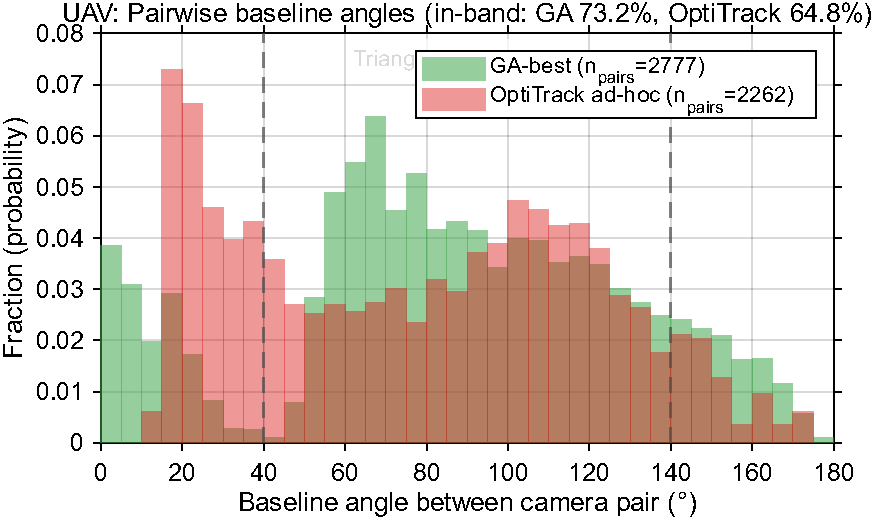
\includegraphics[width=\textwidth]{figures/BaselineAngles_GAvsOpti_UAV.pdf}
\caption{UAV target.}
\label{fig:baseline-uav}
\end{subfigure}
\hfill
\begin{subfigure}{0.49\textwidth}
\centering
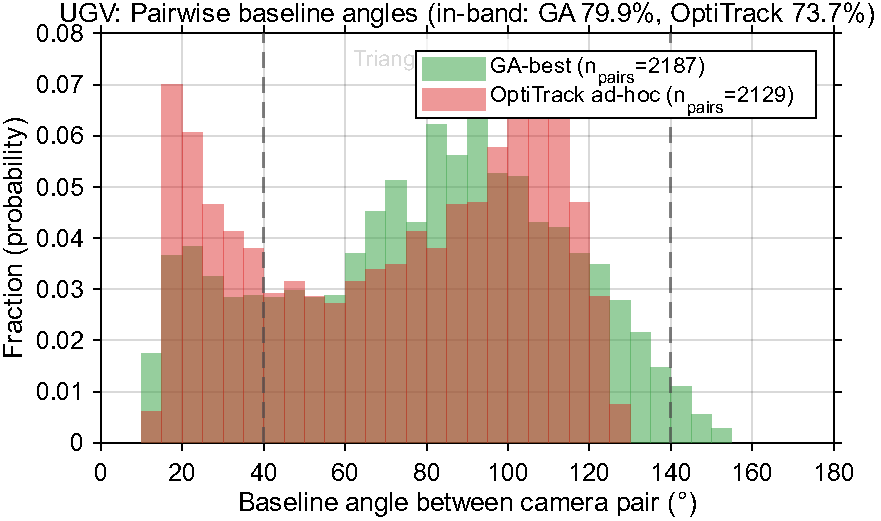
\includegraphics[width=\textwidth]{figures/BaselineAngles_GAvsOpti_UGV.pdf}
\caption{UGV target.}
\label{fig:baseline-ugv}
\end{subfigure}
\caption{Distribution of pairwise camera baseline angles for the GA-best (green) and OptiTrack ad-hoc (red) configurations. Dashed lines mark the triangulability bounds $[40^\circ, 140^\circ]$. The GA shifts pairs into the well-conditioned interior of the band; the ad-hoc layout retains a large near-parallel peak below the lower bound.}
\label{fig:baseline}
\end{figure*}

\begin{figure*}[t]
\centering
\begin{subfigure}{0.49\textwidth}
\centering
\includegraphics[width=\textwidth]{figures/CostField_GAvsOpti_UAV.pdf}
\caption{UAV full-volume.}
\label{fig:costfield-uav}
\end{subfigure}
\hfill
\begin{subfigure}{0.49\textwidth}
\centering
\includegraphics[width=\textwidth]{figures/CostField_GAvsOpti_UGV.pdf}
\caption{UGV ground slab.}
\label{fig:costfield-ugv}
\end{subfigure}
\caption{Spatial distribution of the resolution-uncertainty (top of each panel) and dynamic-occlusion (bottom) components of $J$ across the target grid. The GA layout (left of each panel) produces uniformly low cost; the ad-hoc layout (right) exhibits localised high-cost regions where the placement fails to provide a triangulable view.}
\label{fig:costfield}
\end{figure*}

\subsection{Coverage}
Across the seven-camera, $\Delta=1\,\text{m}$ cells the GA layouts cover $\geq 99.99\,\%$ of target points with at least one camera and $79.6$--$87.2\,\%$ with two or more cameras, against $73.4\,\%$ ($2+$-cam) for the ad-hoc UAV layout, which also leaves $8.4\,\%$ of UAV target points entirely unobserved. Average per-target coverage under the GA layouts is $3.85$--$4.65$ cameras.

\subsection{Computational Cost}
Median per-run wall-clock time at $\Delta=1\,\text{m}$ on $24$ parallel workers is $\sim 20.8\,\text{min}$ (UAV, $\sim 405$ target points) and $\sim 13.6\,\text{min}$ (UGV, $\sim 243$ target points). The dependence on camera count between $k=6$ and $k=8$ is mild ($<30\,\%$), since per-point evaluation cost is dominated by pairwise visibility, range, and triangulability tests rather than by $\mathcal{O}(k)$ FOV checks. A grid-spacing sensitivity sweep ($\Delta \in [0.1, 3]\,\text{m}$) confirms that the chosen $\Delta=1\,\text{m}$ deviates by $\leq 5\,\%$ from the $\Delta=0.1\,\text{m}$ reference on the combined cost whilst delivering a $\sim 250\times$ speedup, defending the discretisation choice.

\subsection{Local Sensitivity}
Fig.~\ref{fig:anglesensitivity} probes the local cost surface by perturbing one camera's roll, pitch, and yaw individually across $\pm 45^\circ$ from the GA-best, with the remaining cameras held fixed. The UAV configuration produces V-shaped cost curves with a clear minimum at zero perturbation in all three axes. The UGV configuration produces asymmetric V's: positive perturbations rotate the probe camera off the floor slab and incur a steep cost rise, whereas negative perturbations point it further into the already-covered region and produce only a shallow rise. The absence of any lower-cost configuration within $\pm 10^\circ$ in any axis confirms that the returned configuration sits at a true local minimum of the cost surface rather than at an arbitrary point the operator schedule happened to abandon.

\begin{figure*}[t]
\centering
\begin{subfigure}{0.49\textwidth}
\centering
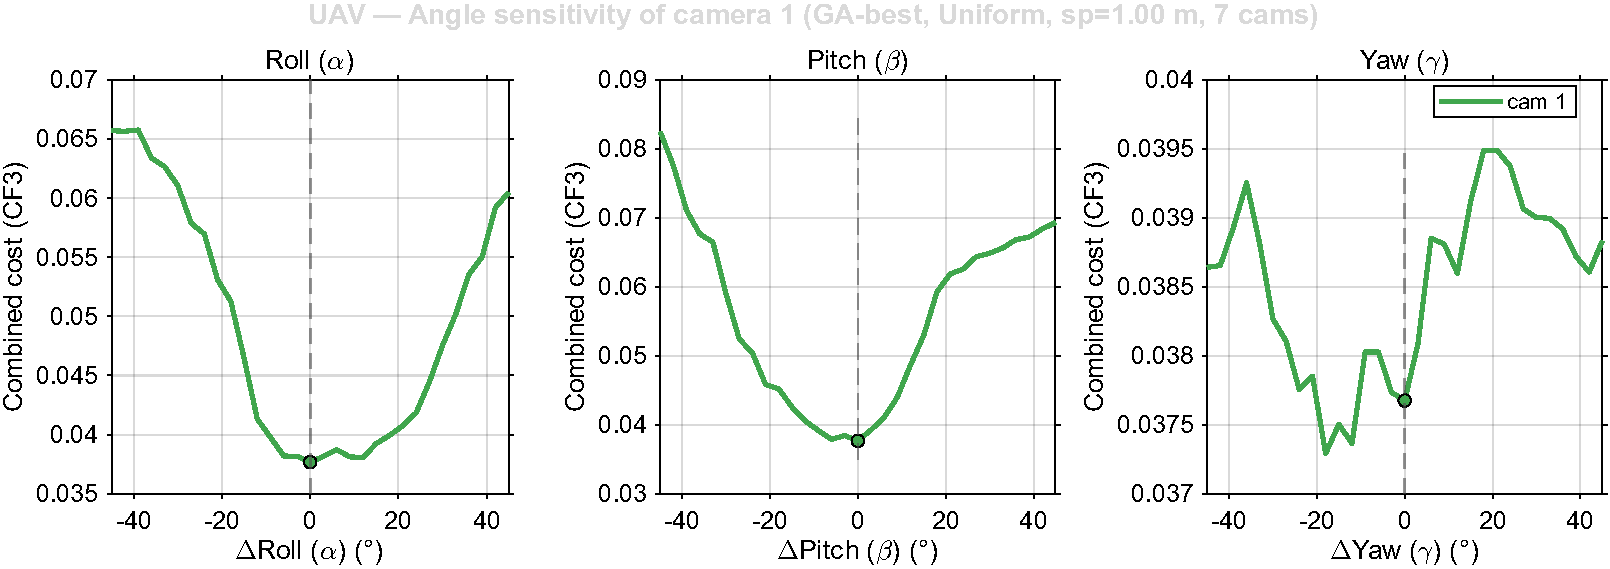
\includegraphics[width=\textwidth]{figures/AngleSensitivity_UAV_cam1.pdf}
\caption{UAV target.}
\label{fig:angle-uav}
\end{subfigure}
\hfill
\begin{subfigure}{0.49\textwidth}
\centering
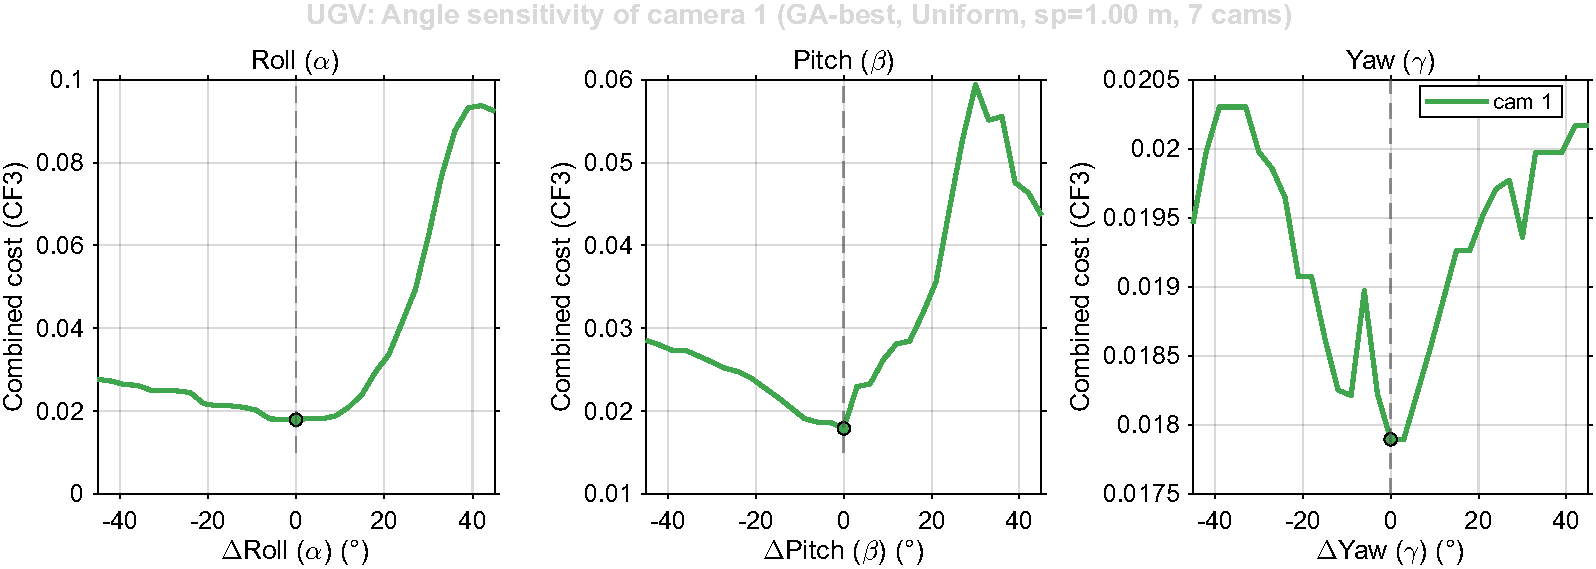
\includegraphics[width=\textwidth]{figures/AngleSensitivity_UGV_cam1.pdf}
\caption{UGV target.}
\label{fig:angle-ugv}
\end{subfigure}
\caption{Combined cost $J$ as camera 1's roll, pitch, and yaw are perturbed individually by $\pm 45^\circ$ from the GA-best, holding the other six cameras fixed. Each curve has a clear minimum at zero perturbation; the UGV curves are asymmetric, reflecting the spatially restricted floor-slab target.}
\label{fig:anglesensitivity}
\end{figure*}

\section{Conclusion and Future Work}
\label{sec:conclusion}
Optimising camera placement is not optional; it should be a prerequisite for accurate tracking.


\begin{thebibliography}{00}

\bibitem{sharma_analysis_1998}
R. Sharma, ``Analysis of uncertainty bounds due to quantization for three-dimensional position estimation using multiple cameras,'' \textit{Optical Engineering}, vol. 37, no. 1, p. 280, Jan. 1998, doi: 10.1117/1.601615.

\bibitem{chen_camera_2000}
X. Chen and J. Davis, ``Camera placement considering occlusion for robust motion capture,'' Stanford Univ., Computer Graphics Laboratory, Tech. Rep., 2000.

\bibitem{olague_optimal_2002}
G. Olague and R. Mohr, ``Optimal camera placement for accurate reconstruction,'' \textit{Pattern Recognition}, vol. 35, no. 4, pp. 927--944, Apr. 2002, doi: 10.1016/S0031-3203(01)00076-0.

\bibitem{chen_occlusion_2008}
X. Chen and J. Davis, ``An occlusion metric for selecting robust camera configurations,'' \textit{Machine Vision and Applications}, vol. 19, no. 4, pp. 217--222, Jul. 2008, doi: 10.1007/s00138-007-0094-y.

\bibitem{zhao_approximate_2013}
J. Zhao, R. Yoshida, S.-c. S. Cheung, and D. Haws, ``Approximate techniques in solving optimal camera placement problems,'' \textit{International Journal of Distributed Sensor Networks}, vol. 9, no. 11, p. 241913, Nov. 2013, doi: 10.1155/2013/241913.

\bibitem{rahimian_optimal_2017}
P. Rahimian and J. K. Kearney, ``Optimal camera placement for motion capture systems,'' \textit{IEEE Transactions on Visualization and Computer Graphics}, vol. 23, no. 3, pp. 1209--1221, Mar. 2017, doi: 10.1109/TVCG.2016.2637334.

\bibitem{aissaoui_designing_2018}
A. Aissaoui, A. Ouafi, P. Pudlo, C. Gillet, Z.-E. Baarir, and A. Taleb-Ahmed, ``Designing a camera placement assistance system for human motion capture based on a guided genetic algorithm,'' \textit{Virtual Reality}, vol. 22, no. 1, pp. 13--23, Mar. 2018, doi: 10.1007/s10055-017-0310-7.

\bibitem{ziegler_optimal_2023}
J. Ziegler, H. Gattringer, and A. M\"{u}ller, ``Optimal camera placement for maximized motion capture volume and marker visibility,'' in \textit{Advances in Service and Industrial Robotics}, T. Petri\v{c}, A. Ude, and L. \v{Z}lajpah, Eds. Cham: Springer Nature Switzerland, 2023, pp. 45--52, doi: 10.1007/978-3-031-32606-6\_6.

\bibitem{corke_petercorkervc3-python_2026}
P. Corke, ``petercorke/RVC3-python,'' GitHub repository, 2026. [Online]. Available: https://github.com/petercorke/RVC3-python

\end{thebibliography}

\end{document}
